%!TEX program = lualatex
% SPDX-License-Identifier: CC-BY-SA-4.0
% latex-atlas 03: monochrome data chart. Bars differ by hatch angle and
% density, never by colour fill; values also appear as figures in a table.
\documentclass[11pt]{article}

\usepackage{iftex}
\ifLuaTeX\else
  \PackageError{latex-atlas}{This example requires LuaLaTeX}
    {Run lualatex, not pdflatex.}
\fi

\usepackage{fontspec}
\usepackage{xcolor}
\usepackage{geometry}
\usepackage{tikz}
\usetikzlibrary{patterns.meta}
\usepackage[tracking=true,protrusion=false,expansion=false]{microtype}

\defaultfontfeatures{Renderer=HarfBuzz}
\IfFontExistsTF{EB Garamond}{
  \setmainfont{EB Garamond}[Numbers={OldStyle,Proportional}]
  \newfontfamily\tablefont{EB Garamond}[Numbers={Lining,Tabular}]
}{
  \setmainfont{TeX Gyre Pagella}[Numbers={OldStyle,Proportional}]
  \newfontfamily\tablefont{TeX Gyre Pagella}[Numbers={Lining,Tabular}]
}

% Paper tint is per-example tuning for this chart plate, not a shared
% token yet; the three examples deliberately differ slightly (see README).
\definecolor{chartpaper}{HTML}{F4EAD8}
\definecolor{ink}{HTML}{25201B}
\pagecolor{chartpaper}
\color{ink}
\geometry{a4paper,top=20mm,bottom=20mm,left=24mm,right=24mm}
\pagestyle{empty}

\tikzset{
  bar/.style={draw=ink,line width=0.55pt},
  hatchA/.style={pattern={Lines[angle=45,distance=3pt,line width=0.35pt]},pattern color=ink},
  hatchB/.style={pattern={Lines[angle=-45,distance=3pt,line width=0.35pt]},pattern color=ink},
  hatchC/.style={pattern={Lines[angle=90,distance=2.6pt,line width=0.3pt]},pattern color=ink},
  hatchD/.style={pattern={Hatch[distance=3.2pt,line width=0.25pt]},pattern color=ink}
}

\begin{document}

\begin{center}
  {\small\textls[110]{\textsc{Table III}}}\par
  \vspace{0.3em}
  {\Large Coals Raised, in Thousands of Tons}\par
  \vspace{0.2em}
  {\itshape four pits, 1869--1873; tone by hatch, value by height}
\end{center}

\vspace{1em}

\begin{center}
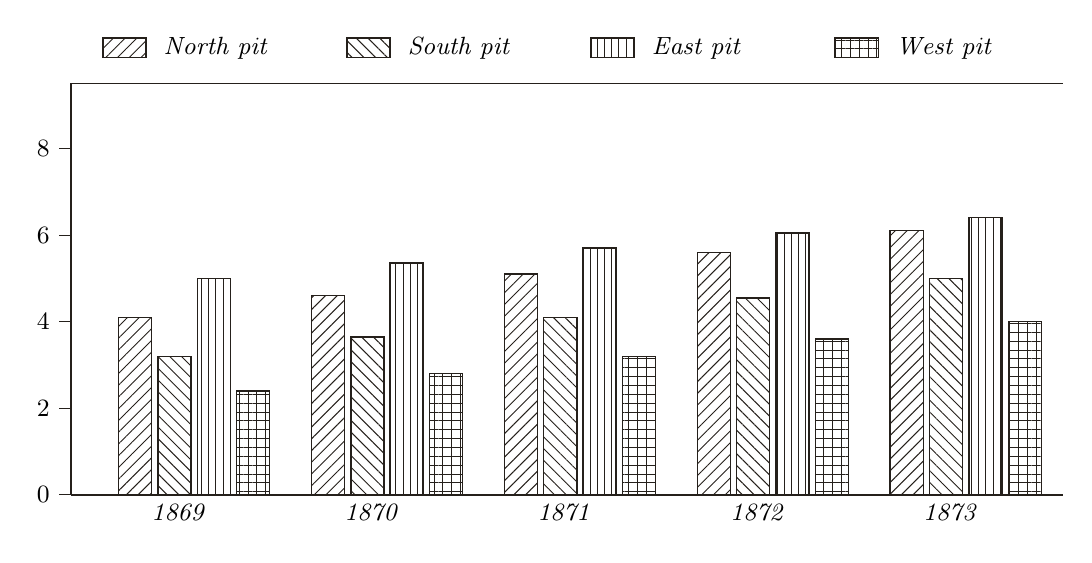
\begin{tikzpicture}[x=1cm,y=0.55cm]
  % Axes.
  \draw[ink,line width=0.6pt] (0,0) -- (0,9.5) -- (12.6,9.5);
  \draw[ink,line width=0.6pt] (0,0) -- (12.6,0);
  \foreach \y in {0,2,4,6,8} {
    \draw[ink,line width=0.35pt] (0,\y) -- (-0.15,\y);
    \node[left,font=\small] at (-0.15,\y) {\y};
  }
  % Four groups of five yearly bars; hatch identifies the pit.
  \foreach \g/\lab in {0/1869,1/1870,2/1871,3/1872,4/1873} {
    \pgfmathsetmacro{\x}{\g*2.45+0.6}
    \node[below,font=\small\itshape] at (\x+0.75,0) {\lab};
    \draw[bar,hatchA] (\x,0) rectangle +(0.42,{4.1+0.5*\g});
    \draw[bar,hatchB] (\x+0.5,0) rectangle +(0.42,{3.2+0.45*\g});
    \draw[bar,hatchC] (\x+1.0,0) rectangle +(0.42,{5.0+0.35*\g});
    \draw[bar,hatchD] (\x+1.5,0) rectangle +(0.42,{2.4+0.4*\g});
  }
  % Legend: hatch swatches, no colour.
  \foreach \i/\sty/\lab in {
    0/hatchA/North pit, 1/hatchB/South pit,
    2/hatchC/East pit, 3/hatchD/West pit} {
    \pgfmathsetmacro{\lx}{0.4+\i*3.1}
    \path[\sty] (\lx,10.1) rectangle +(0.55,0.45);
    \draw[bar] (\lx,10.1) rectangle +(0.55,0.45);
    \node[right,font=\small\itshape] at (\lx+0.65,10.32) {\lab};
  }
\end{tikzpicture}
\end{center}

\vspace{1em}

\begin{center}
\tablefont\small
\begin{tabular}{@{}lrrrrr@{}}
\textsc{Year} & \textsc{North} & \textsc{South} & \textsc{East} & \textsc{West} & \textsc{Total}\\
\hline
1869 & 410 & 320 & 500 & 240 & 1470\\
1870 & 460 & 365 & 535 & 280 & 1640\\
1871 & 510 & 410 & 570 & 320 & 1810\\
1872 & 560 & 455 & 605 & 360 & 1980\\
1873 & 610 & 500 & 640 & 400 & 2150\\
\end{tabular}
\end{center}

\vspace{0.8em}
\footnotesize\noindent
Hatch angle carries the series, bar height the value, figures the record.
No grey fill is used, so the plate survives monochrome reproduction; the
table repeats every plotted number for the reader who measures with a
rule rather than an eye.

\end{document}
